\documentclass[12pt]{article}
\usepackage{tikz}
\usetikzlibrary{shapes,snakes}
\usetikzlibrary{arrows,automata}
\usepackage{algorithm}
\usepackage{algorithmic}
\usepackage{graphicx} 
\usepackage{fancybox}
\usepackage{setspace}  
\usepackage[colorlinks,linkcolor=blue,citecolor=magenta]{hyperref}
\usepackage{enumerate} 
\usepackage{amsthm,amssymb,amsmath}
\usepackage{indentfirst}
\usepackage{listings}
\usepackage{alltt}
\usepackage{clrscode}
\renewcommand{\algorithmiccomment}[1]{// #1}
\newtheorem{theorem}{Theorem}
\begin{document}

\title{Initial Value Computation}
\author{}
\date{\today}
\maketitle
\newcommand{\dom}{\textsf{dom}}

\section{Definitions}
In this draft we want to explain the notion of domains in DBToaster calculus \cite{1}. DBToaster uses query language AGCA(which is stands for AGgregation CAlculus). 
AGCA expressions are built from constants, variables, relational atoms, aggregate sums (Sum), conditions, and variable assignments ($\gets$) using ``+''  and ``$\cdot$''. The abstract syntax can be given by the EBNF:
\begin{equation}
\label{def:agca}
q\text{ ::- }q\cdot q | q + q|v \gets q |v_{1}\theta v_{2}|R(\vec{y})|\text{c}|\text{v}|(M[\vec{x}][\vec{y}]\text{::-}q)
\end{equation}
The above definition can express all SQL statements. Here $v$ denotes variables, $\vec{x},\vec{y}$ tuples of variables, $R$ relation names, $c$ constants, and $\theta$ denotes comparison operations $(=,\neq, >, \geq, <, \text{ and }\leq)$.
 ``+'' represents unions and ``$\cdot$'' represents joins. Assignment operator($\gets$) takes an query and assigns its result to a variable($v$). A map $M[\vec{x}][\vec{y}]$ is a subquery with some input($\vec{x}$) and output($\vec{y}$) variables. It can be seen as a nested query that for the arguments $\vec{x}$ produces the output $\vec{y}$, it is not defined in \cite{1} but we added here for the purpose of this work.

The domain of a variable is the set of values that it can take. The domain of all the variables in a query expression can easily be computed recursively if some rules are respected. We will use through out the entire paper the notation of $\text{\dom{}}_{\vec x}(q)$ for the domain of a set of variables, where $q$ is the given query and $\vec x$ is a vector representing the variables(not necessarily present in the expression $q$). We will start by saying the $\vec x=<x_1,x_2,x_3,\cdots,x_n>$ will be the schema of all the variables and that $\vec c=<c_1,c_2,c_3,\cdots,c_n>$ will be the vector of all constants, that will match the schema presented by $\vec x$. It is not necessary that $\vec{x}$  has the same schema as the given expression. We will give the definition of $\dom{}_{\vec x}(R(\vec y))$:

%\begin{equation}
%\label{def:relation}
%\dom{}_{\vec x}(R(\vec y))=\bigg\{\vec %c\,\Big|\,(\prod_{i:x_{i}\in \vec y}^{}(x_{i}\gets %c_{i})\cdot R(\vec y))\not= 0\bigg\}
%\end{equation}

\begin{equation}
\label{def:relation}
\dom{}_{\vec x}(R(\vec y))=\bigg\{\vec c\,\Big|\,\sigma_{\forall x_i\in(\vec{x}\cap\vec{y}): x_{i}=c_{i}}R(\vec y)\not= \const{NULL}\bigg\}
\end{equation}

Thus, we can evaluate $\text{\dom}_{\vec{x}}$ for a broader range of $\vec{x}$ and it is not restricted by the schema of the input query expression. In such cases the \dom{} is infinite as the not presenting variables in the query can take any value.

For the comparison operator ($v_{1}\theta v_{2}$), where $v_1$ and $v_2$ are variables, we can compute the domain as follows:
%\begin{equation}
%\text{\dom{}}_{\vec{x}}(v_{1}\theta v_{2})=\bigg\{\vec{c}\,\Big|\,\Big(\big(\prod_{i}(x_{i}\gets c_{i})\big)(v_{1}\theta v_{2})\Big)\not= 0\bigg\}
%\end{equation}

\begin{equation}
\text{\dom{}}_{\vec{x}}(v_{1}\theta v_{2})=\bigg\{\vec{c}\,\Big|\,\forall i,j:(v_{1}=x_{i}\land v_{2}=x_{j})\Rightarrow c_{i}\theta c_{j}\bigg\}
\end{equation}

The domain of a comparison is infinite.

For the join operator we can write:
\begin{equation}
\label{def:join}
\text{\dom{}}_{\vec{x}}(q_{1}\cdot q_{2})=\{\vec{c}\,|\vec{c}\in\text{\dom{}}_{\vec{x}}(q_{1})\land\vec{c}\in\text{\dom{}}_{\vec{x}}(q_{2})\}
\end{equation}
while for the union operator the domain definition is very similar:
\begin{equation}
\label{def:plus}
\text{\dom{}}_{\vec{x}}(q_{1}+ q_{2})=\{\vec{c}\,|\vec{c}\in\text{\dom{}}_{\vec{x}}(q_{1})\lor\vec{c}\in\text{\dom{}}_{\vec{x}}(q_{2})\}
\end{equation}
\begin{eqnarray}
\dom{}_{\vec x}(constant)=\Big\{\vec c\Big\}\label{def:const}\\
\dom{}_{\vec x}(variable)=\Big\{\vec c\Big\}\label{def:var}
\end{eqnarray}
In \eqref{def:const},\eqref{def:var} and \eqref{def:null} $\vec{c}$ stands for all possible tuples match schema of $\vec{x}$, so the domains in these two cases are infinite. 
Finally, we can give a formalism for expressing the domain of a variable that will participate in an assignment operation:
%\begin{equation}
%\label{assign1}
%\text{\dom{}}_{\vec{x}}(v\gets q_{1})=\bigg\{\vec{c}\,\Big|\vec{c}\in\text{\dom{}}_{\vec{x}}(q_{1})\land \bigg(\forall i:(x_{i}=v)\Rightarrow\Big(\big(q_{1}\cdot\prod_{j:x_{j}\neq v } (x_{j}=c_{j})\big)=c_{i}\Big)\bigg)\bigg\}
%\end{equation}
\begin{equation}
\label{assign2}
\text{\dom{}}_{\vec{x}}(v\gets q_{1})=\Big\{\vec{c}\Big|\vec{c}\in\text{\dom{}}_{\vec{x}}(q_{1})\land \big(\forall i,j: (x_{i}=v=x_{j})\Rightarrow(c_{i}=c_{j}=q_{1})\big)\Big\}
\end{equation}
In fact using implication operator in the above definition allows us to extend the $\vec{x}$ to whatever vector we want, as we already said the schema of $\vec{x}$ is not necessarily the same as the schema of $q$. %Here is a mathematical reformulation of \eqref{assign1}:
For the sake of completeness we define the domain of empty set as infinite:
\begin{equation}
\label{def:null}
\text{\dom}_{\vec{x}}(\const{NULL})=\{\vec{c}\}
\end{equation}

\section{Computing the arities of the AGCA expressions}
Having the definitions for the domains, we will try to give some insight regarding to the notion of arity. We will start with an example relation: $$q=R(a,b)\cdot S(b,c)$$ the schema for q will have three variables $(a,b,c)$. The arity of a tuple is the number of its occurrences in the relation, in other words the order of multiplicity of that tuple. The arity of a tuple will increase or decrease if insertions or respectively deletions will be made to a relation. For example:
\begin{table}[ht]
\centering
\begin{tabular}{c c c c}
	R & a & b & arity\\ [0.2ex]
	%heading
	\hline
	  & $<$1 & 2$>$ & 1 \\
	  & $<$1 & 3$>$ & 2 \\
	  & $<$3 & 4$>$ & 1 \\
\end{tabular}
\caption{Relation $R$}
\end{table}
\begin{table}[ht]
\centering
\begin{tabular}{c c c c}
	S & b & c & arity\\ [0.2ex]
	%heading
	\hline
	  & $<$1 & 1$>$ & 1 \\
	  & $<$2 & 2$>$ & 2 \\
	  & $<$3 & 5$>$ & 2 \\
\end{tabular}
\caption{Relation $S$}
\end{table}
\begin{table}[ht]
\centering
\begin{tabular}{c c c c c}
	$R\cdot S$ & a & b & c & arity\\ [0.2ex]
	%heading
	\hline
	  & $<$1 & 2 & 2$>$ & 2 \\
	  & $<$1 & 3 & 5$>$ & 4 \\
	  & $<$3 & 4 & $*>$ & 0 \\
	  & $<*$ & 1 & 1$>$ & 0 \\
\end{tabular}
\caption{Relation $R\cdot S$}
\end{table}

We need to maintain the maps for certain values as long as the arity of a tuple is greater then 0. If the arity  of the tuple drops to 0 then the tuple will not be taken into consideration and therefore it can be eliminated from the domains of the maps.

We need to store the arities inside each map and also way to compute the arity of an AGCA expression. Since we substitute the subexpressions with maps, we can easily consider the relations as the maps without input variables. Also a map with input variables can be seen as a relation with a group-by clause. Input variable of a map bind some variables. Thus if we compute the map values by all different combinations of these variables, we will look up into these values and return the appropriate value according to the input variables.  

We define the function \emph{arity} which will be used to compute the arity of a tuple in a certain relation. The function will be defined on the relation and the tuple for which the multiplicity order is desired to be computed. $$arity(\text{Relation } q,\text{Tuple } t)=\text{multiplicity order of }t\text{ in the } q =\pi_{t}(q)$$ where $\pi_{t}(q)$ means the projection of relation $q$ for the tuple $t$. This function can be used for the computation of the arity of the expressions from the AGCA: $q\text{ ::- }q\cdot q\text{ }|\text{ }q+q\text{ }|\text{ }q \theta t\text{ }|\text{ }t\gets q\text{ }|\text{ constant}\text{ }|\text{ variable}$. However constants and variables can be eliminated from the computation because relations are of interest.

\begin{align}
arity(q_{1}\cdot q_{2},t)&=\sum\limits_{\{t_{1}\}\Join \{t_{2}\}={t}}^{}arity(q_{1},t_{1})*arity(q_{2},t_{2})\\
arity(q_{1} + q_{2},t)&=arity(q_{1},t)+arity(q_{2},t)\text{, where Schema}(q_{1})\\=\text{Schema}(q_{2})\\
arity(v_1\text{ } \theta \text{ } v_2,t)&=\begin{cases}1,& \mbox{if } v_1\theta v_2 \mbox{ is true and }v_{1}\in t \land v_{2}\in t\\
0,& \text{otherwise} \mbox{ is false} 
\end{cases}\\
arity(v\gets q,t)&=\begin{cases}0, \mbox{ if $t\setminus\{v\}\not\in \text{\dom}_{Schema(t)}(q)$}\\ 1, \mbox{ otherwise} \end{cases}
\end{align}

%\section{Graph representation of maps}
%For computing the domains of input variables of maps we can use graph modeling. In such a way that, given the expression we can compute the domain of each expression with this modeling in $O(m\cdot p)$ where $m$ is the number of occurrences of all input variables and $p$ is the cost of evaluating the domains according to the mentioned rules. \\
%\par
%In this section firstly we talk about the the graph modeling(dependency graph), then we will give an algorithm for computing this dependency graph from the parse tree of expressions. 
%From the parse tree of an expression we can construct a directed graph $G(V,E)$. For each map $m[.][.]$ there is a vertex in $V$ and edges represent the variable. We have an edge between $m_{1}$ and $m_{2}$ with label $a$, if and only if $a$ is in the input variables of $m_{2}$ and output variables of $m_{1}$ and there is an information flow from $m_{1}$ to $m_{2}$. \\
%\par
%Obviously this graph does not have any cycle. To prove it, suppose it has a cycle with at least two vertices, call the first two vertices as $m_{1},m_{2}$. In the cycle there is an edge between $m_{1}$ and $m_{2}$. Since this is a cycle then there is a path between $m_{2}$ and $m_{1}$ also. But it is not possible because having an edge between $m_{1}$ and $m_{2}$ means that $m_{2}$ occurs after $m_{1}$ and according to information flow rule we can not have a path again between $m_{2}$ and $m_{1}$. \\
%\par
%In this graph vertices without any incoming edge are always the relations. If we evaluate the nodes with a topological traversal we can guarantee that the input variables of each maps is computed in order. The cost of domain computations is $O(m\cdot p)$, where $m$ is the number of edges in the graph and $p$ is the cost of using any of mentioned rules for computing the domain of subexpressions as we had in the aforementioned way. \\
%\par
%We can construct the graph from the given parse tree in $O(m)$ where $m$ is the number of edges. We start from the root of the parse tree and recursively compute the subgraph of the left child and right child, then we add the edges between the maps with some input variables on the right child to the appropriate vertices on the left child's graph. Since we consider each edge just one time in the algorithm, the overall order is $O(m)$. 

\section{Domain computation}

We are trying to compute the domain of variables that appear in queries. This computation is performed on the parse tree. We can traverse the tree in post order, first visiting the leaves that are represented by some relations and afterwards visiting the parent nodes and combining the relations of the children nodes. Using this technique we are trying to compute the domains, but also the vector $\vec x$ of all the variables defined in that query.

The intuition behind the algorithm is simple. For computing the domain of a node we first compute the domain of its left child and according to the operator of the node itself we decide how to send the information from left child to right child, and then the domain of the right child.

The algorithm needs as inputs the root of the tree and a structure that must be previously defined and returns a structure that contains the vector of variables($\vec{x}$) and the domains for each variable defined in the vector(\dom). The structure will look like:

\begin{alltt}
struct \{
x: the vector of all the variables 
dom: the domains of all the variables
\}
\end{alltt}

In Algorithm \ref{alg1} we define function \textsf{computeDomain} which helps us to compute the domains for variables within a given query. When invoking the function, we pass as arguments of the function, the root of the parse tree and a structure which will have the vector of variables and the domain of the variables as nil, \textsf{computeDomain}$(root,s)$.
\par
In Algorithm~\ref{alg1} we have a variable $node$ which represents a node in the parse tree. It has 2 children which can be accessed by fields $left, right$. Also each node has a type field, which can be accessed by $type$. A type of a node can be any of different types in definition~\eqref{def:agca}. Each node has boolean field($isMap$) which indicates if it is representing a map or not. 
For representing the maps we need another global structure for storing the properties of each map. Here we use $Maps$ as an associated array whose keys are the nodes and the values are the domain of the input parameters to the map(accessible via field $\vec{x}$) and the domain of its output variables(accessible via $\vec{y}$). 

\begin{algorithm}[H]
\caption{computeDomains($node$,$s$)} 
\label{alg1}
\textbf{Input:} $node$ as the root of the tree to be traversed, and $s$ as the structure \\
\textbf{Output:} a structure $result$ that will contain the vector of variables $\vec x$ and the domains of each variable $\dom{}_{\vec x}(query)$
\begin{algorithmic}[1]
\IF{$node.type=$``+''}
\STATE  $s_{1}\gets$ computeDomain($node$.$left, s$)
\STATE  $s_{2}\gets$ computeDomain($node.right, s$)
\STATE  $result.\vec{x}\gets s_{1}.\vec{x} \cup s_{2}.\vec{x}$ \COMMENT{this will compute the vector for all the variables, both from the right and left node}
\STATE  $result.dom\gets \text{\dom}_{result.\vec x}(node.left + node.right)$
\ELSIF{$node.type=$``*''}
\label{line:join1}
\STATE  $s_{1} \gets \text{computeDomain}(node.left, s)$
\label{line:join2}
\STATE $result\gets$ computeDomain$(node.right, s_{1})$
\ELSE 
\label{line10}
\STATE $result.\vec{x}\gets s.\vec{x} \cup \{\text{all the variables of the $node$}\}$
\STATE $result.dom\gets \text{\dom}_{result.\vec{x}}(s.dom)\cap\text{\dom}_{result.\vec{x}}(node)$\label{line2}
\ENDIF
\IF{$node.isMap=$ \TRUE}
\STATE $Maps[node].\vec{x}\gets\text{\dom}_{\vec{x}}(s.dom)$
\STATE $Maps[node].\vec{y}\gets result$
\ENDIF
\RETURN $result$
\end{algorithmic}
\end{algorithm}
The order of Algorithm \ref{alg1} is $O(n\cdot P)$ where $n$ is the number of nodes in the parse tree and $P$ is the time needed for any rule of \dom{}'s computation, according to previous section. Clearly this algorithm visits each node only one time. \par

In Algorithm \ref{alg1} we suppose that there are three types of nodes: union nodes that represent $q+q$ expressions, join nodes that represent $q*q$ expressions and the other remaining node types. If a node represents a map we show it like $M[\vec x][\vec y]$. In addition to nodes, we have three types of leaves: simple relations $R(\vec y)$, inequalities $v_{1}\theta v_{2}$ and assignment relations $v \gets q$. A union node or a join node will always have two children, therefore the line \ref{line10} will be executed when a leaf is visited. When a node that is represented by a map, is encountered then the algorithm should produce a set of variables and respectively the domains of each variable. Also in line \ref{line2} we use the definition of \dom{} to extend its schema to a broader range according to what was said in the previous section, definition \eqref{def:relation}. \\\par

In line~\ref{line2} we take the domain of a domain. We use this for extending the domain regarding to a new schema vector $\vec x$. In other words we add some other variables to the vector and therefore compute the domain for each variable within that vector. Without loss of generality, we can consider a domain as a set with schema or a relation. So we can easily extend the domain of a set to a broader set of variables with the definition of the domain or a relation in \eqref{def:relation}. 

\begin{figure}[htbp]
\begin{center}
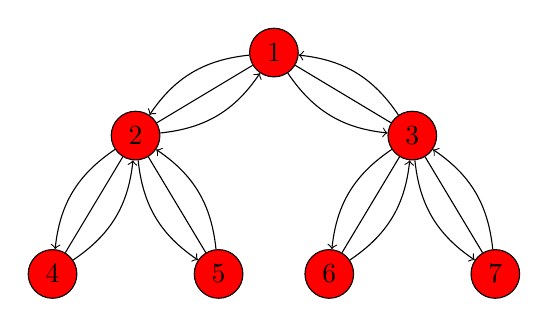
\begin{tikzpicture}%[level/.style={sibling distance=40mm,level distance=15mm}]
[level 1/.style={circle, draw,scale=1.0, fill=red,
    level distance=30pt, sibling distance=100pt},
    level 2/.style={circle, draw, scale=1.0,
    level distance=50pt, sibling distance=60pt}]
    \tikzstyle{every node}=[circle,draw,fill=red]
    \node[] (a){1}
        child { 
            node [](b){2}
            child{node(d){4}}
            child{node(e){5}} 
        }
        child { 
        		node[] (c){3}
		child{node[](f){6}}
		child{node(g){7}}
	};
	\draw[->] (a) to [bend right=25](b);
	\draw[->] (b) to [bend right=25](a);
	
	\draw[->] (a) to [bend right=25](c);
	\draw[->] (c) to [bend right=25](a);
	
	\draw[->] (b) to [bend right=25](d);
	\draw[->] (d) to [bend right=25](b);
	\draw[->] (b) to [bend right=25](e);
	\draw[->] (e) to [bend right=25](b);
	\draw[->] (c) to [bend right=25](f);
	\draw[->] (f) to [bend right=25](c);
	\draw[->] (c) to [bend right=25](g);
	\draw[->] (g) to [bend right=25](c);
	
\end{tikzpicture}
\end{center}
\caption{Tree traversal}
\label{fig1}
\end{figure}

	The algorithm starts with node 1, which represents the root of the parse tree. It recursively goes through each of the leaves, therefore constructs the variable vector and also the domain for each variable.
	
	It is known that the left most leaf will always be a relation that produces only output variables. Otherwise, if this condition is not sustained then it will contradict the rules imposed by the DBToaster calculus. Therefore node 4 will always be a simple relation that will give some output variables, which may help in future nodes if those nodes have input variables. If, for example node 5 will have input variables, then those variables will depend only on the output variables that node 4 is giving.
	
	We have mentioned that besides map nodes, there are two more types of nodes: the union node and the join node. When a union node is met, then it is known that domains of variables will not pass over this operator and for that the variables and their domains, which were obtained in the parent, will be passed to each of this node's children, thus applying the distribution rule of join operator over the union operator. For example if we have $ q1 * (q2 * q3 + q4 * q5) \equiv q1 * q2 * q3 + q1 * q4 * q5$, the variables and domain obtained for $q1$ will be passed both to $q2*q3$ and $q3*q4$, without modifying any of the domains, regarding that some domains may change on one branch, for example $q2*q3$. For the other type of node, the join node, the passing of domains is allowed, and therefore a domain can be refined by the relation on the right side of the parent node.
	
	Every time the algorithm encounters a map then it will create the domain for that specific map. Here we can make a difference between input and output variables, because the domain of input variables is dependent on the domains of output variables from the left side of the map's parent node, and the domain of the output variables are going to be produced by the children of the map's node. All this information will be stored in a global variable which can be easily accessed.
\begin{theorem}
Algorithm \ref{alg1} computes the domain of each variables and maps.
\end{theorem}

\begin{proof}

The proof is by induction on the height of the tree. The theorem is held for a tree consisting of only one node. Since this node is a simple relation and the Algorithm \ref{alg1} goes  through lines \ref{line10}-\ref{line2}. As we defined, the domain of any empty set is infinite(all possible values) so the domain is correctly computed in line \ref{line2}.

Now suppose that the Algorithm \ref{alg1} works for all the trees of a height less than $k$. We want to prove that it will work as well for trees of height $k$. Let $T$ be a tree with height $k$. The root should have two children since the construction of the tree only creates nodes with leaves or two children \cite{1}. The height of both of these children should be less than $k$. So we have correctly compute the domain of the left child and its input variable. Now we have two cases, if the root node is a union node or a join node. If this is a union node then we can compute the domain of the right child independently, since no information is passed over the ``+'' in DBToaster\cite{1}. We compute the domain of the root according to definition \eqref{def:plus}. But if the root node is a join node, we have to pass the information from left child to the right child, since the right child may have some input variables which are defined in the left child. This is done in lines \ref{line:join1},\ref{line:join2}.\par
Thus in either of two cases we compute the domain of the root correctly and the theorem follows.
\end{proof}

%The algorithm presented above will compute the domains for each map that is met during the tree traversal. However, if, for example, we want to compute the domain of just one map, then the algorithm can easily be modified to accept this possibility. For example take the next figure \ref{fig2}.
%
%	\begin{figure}[htbp]
%	\begin{center}
%	\begin{tikzpicture}%[level/.style={sibling distance=40mm,level distance=15mm}]
%	[level 1/.style={circle, draw,scale=1.0, fill=red,
%	    level distance=30pt, sibling distance=100pt},
%	    level 2/.style={circle, draw, scale=1.0,
%	    level distance=50pt, sibling distance=60pt}]
%	    \tikzstyle{every node}=[circle,draw,fill=red]
%	    \node[] (a){1}
%	        child { 
%	            node [](b){2}
%	            child{node(d){4:$R(\vec y)$}}
%	            child{node(e){5}} 
%	        }
%	        child { 
%	        		node[] (c){3:$M[\vec x][\vec y]$}
%		};
%		\draw[->] (a) to [bend right=25](b);
%		\draw[->] (b) to [bend right=25](a);
%		
%		\draw[->] (a) to [bend right=25](c);
%		\draw[->] (c) to [bend right=25](a);
%		
%		\draw[->] (b) to [bend right=25](d);
%		\draw[->] (d) to [bend right=25](b);
%		\draw[->] (b) to [bend right=25](e);
%		\draw[->] (e) to [bend right=25](b);
%		
%	\end{tikzpicture}
%	\end{center}
%	\caption{Partial tree seen by the algorithm}
%	\label{fig2}
%	\end{figure}
%Here we want to compute the domain for node $3$. The algorithm will go exactly as the previous one, however the domain for the output variables can not be computed because the algorithm will not see any more children of the node represented by the map. Therefore, the use of this algorithm will produce only the domains for the input variables, because the computation of the domains of the output variables will require the traversal of node's children.
%
%For the algorithm to work, we must add a control variable which could be of boolean type. When invoking the function, the necessary arguments are going to be the root of the parse tree, the structure s, which will have the vector variable and the domains for each variable as nil, and the variable $stop$ which will be transmitted by it's address, not by the value, therefore any change to this variable will be permanently. At first the boolean variable will be $false$, but when the necessary map is encountered then the variable will become true, therefore stopping the process of computing the whole domain for each variable that might appear in the query expression.
%
%\begin{algorithm}[H]
%\caption{computeDomains($node$,$s$,$stop$)} 
%\label{alg2}
%\textbf{Input:} $node$ as the root of the tree, $s$ as the structure, $stop$ a boolean variable that will tell us when the specific map is met\\
%\textbf{Output:} a structure $result$ that will contain the vector of variables $\vec x$ and the domains of each variable $\dom{}_{\vec x}(query)$
%\begin{algorithmic}[1]
%\IF {stop=false}
%\IF{$node.type=$``+''}
%\STATE  $s_{1}\gets$ computeDomain($node.left, s$,$stop$)
%\STATE  $s_{2}\gets$ computeDomain($node.right, s$,$stop$)
%\IF {$s_{2}!=nil$}
%\STATE  $result.\vec{x}\gets s_{1}.\vec{x} \cup s_{2}.\vec{x}$ \COMMENT{this will compute the vector for all the variables, both from the right and left node}
%\STATE  $result.dom\gets \text{\dom}_{result.\vec x}(node.left + node.right)$
%\ELSE 
%\STATE $result \gets s_{1}$
%\ENDIF
%\ELSIF{$node.type=$``*''}
%\STATE $s_{1} \gets \text{computeDomain}(node.left, s,stop)$
%\STATE $s_{2}\gets$ computeDomain$(node.right, s_{1},stop)$
%\IF {$s_{2}!=nil$}
%\STATE $result\gets s_{2}$
%\ELSE
%\STATE $result \gets s_{1}$
%\ENDIF
%\ELSIF {$node.type=M[\vec x][\vec y]$}
%\STATE $result.\dom{}\gets\text{\dom}_{\vec{x}}(s.dom)$
%\STATE $result.\vec{x}\gets \vec x$
%\STATE $stop=true$
%\ELSE 
%\STATE $result.\vec{x}\gets s.\vec{x} \cup \{\text{all the variables of the $node$}\}$
%\STATE $result.dom\gets \text{\dom}_{result.\vec{x}}(s.dom)\cap\text{\dom}_{result.\vec{x}}(node)$
%\ENDIF
%\ELSE
%\STATE $result=nil$
%\ENDIF
%\RETURN $result$
%\end{algorithmic}
%\end{algorithm}

\section{Computing and maintaining the domains using the arities}

The main goal is to maintain the domains of the variables of each map that will be present in query expression. We must offer a solution of maintaining these domains, see how the domains will increase or decrease if tuples are being added or deleted from the relations.

\begin{thebibliography}{9}
\bibitem{1} C. Koch, \emph{Incremental Query Evaluation in a Ring of Databases},  preprint (2011).
\end{thebibliography}
\end{document}




